\section{Design}
\label{design}

When implementing the editor there were a number of design decisions we had to
take to make a concrete implementation of the formal editor described by
Godiksen et al.\pepm. In this section we will discuss the high level design
decision we have taken.


\subsection{Abstract syntax trees}

Since an AST is a tree data structure, there are a multitude of ways we could
visualize them, and we had to pick a number of representations among many. We
are interested in visualizing the AST to make the editor intuitive for a user.
We are not necessarily interested in finding the ``best'' visualization, nor in
implementing a vast number of different representations.

A very simple representation would be to represent the AST in a textual form,
as seen in figure \ref{fig:ast-in-text-form}.

\begin{figure}[H]
    \Large
    \begin{equation*}
      \cursor{(\app{\breakpoint{(\lambda{x}{(\app{x}{x})})}}
      {(\lambda{x}{(\app{x}{x})})})}
    \end{equation*}
    \caption{An AST visualized in textual form.}
    \label{fig:ast-in-text-form}
\end{figure}

The notation used for this representation follows the notation used by Godiksen
et al.~\pepm. We implemented this representation, as it was straightforward to
implement, and it can provide the user with a compact and formal visualization
of the AST. However, this approach comes with some drawbacks. It can be
difficult to reason about, especially as an AST grows large.

Because of this, we decided to implement another representation in addition to
the textual form. The second approach is by representing it as tree structures
often are, i.e. where nodes are rectangles and branches are lines that grow
downwards, as seen in figure \ref{fig:ast_visual_tree}. A potential variation
of this structure, could be in the form of a horizontal tree spanning from left
to right

Switching between the two visualizations is meant to be as easy as a click of a
button, which allows the user to choose their preferred representation at any
time.

\begin{figure*}
  \center
  \noindent\begin{minipage}{.45\textwidth}
    \center
    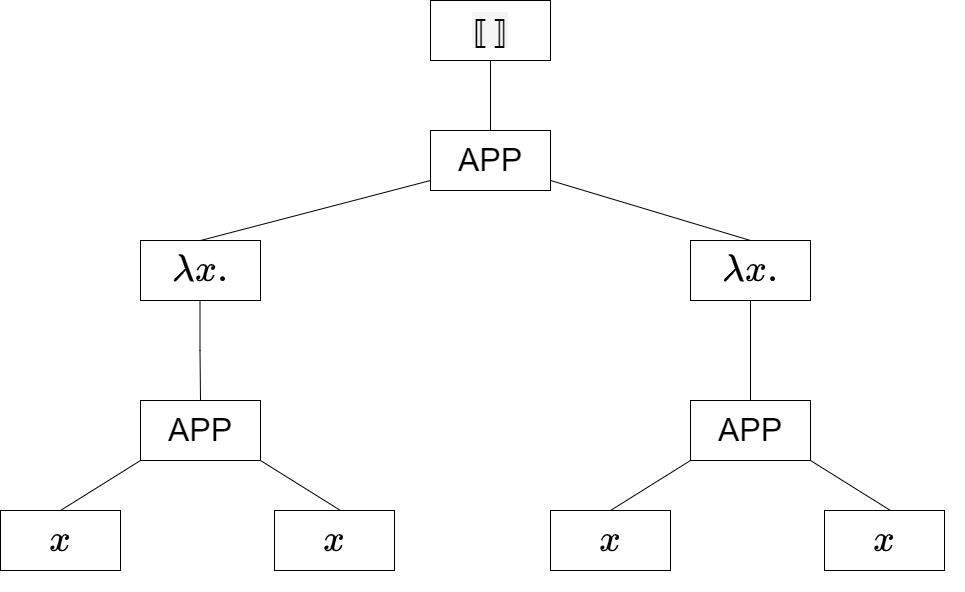
\includegraphics[width=\textwidth]{assets/ast_root_cursor.png}
  \end{minipage}\hfill
  \begin{minipage}{.45\textwidth}
    \center
    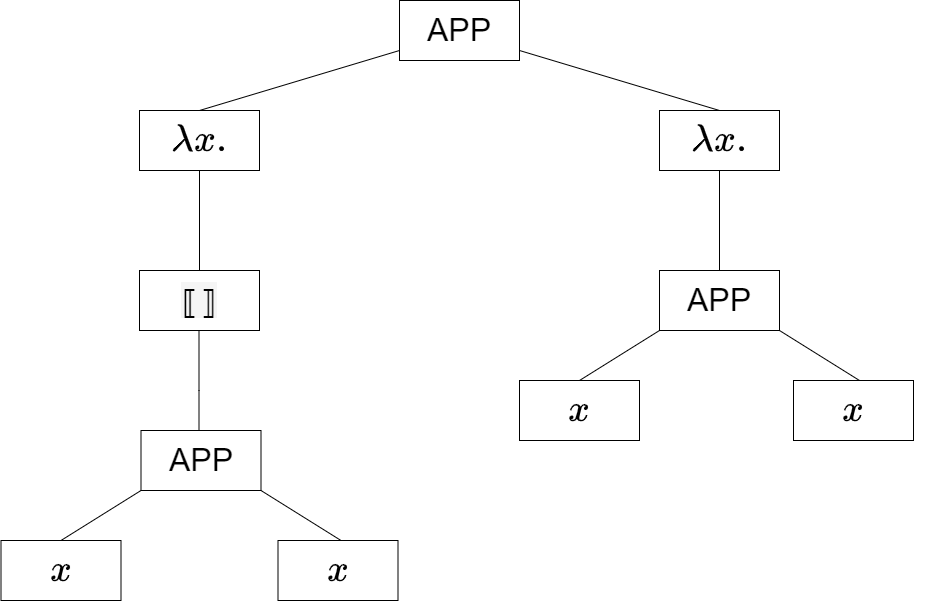
\includegraphics[width=\textwidth]{assets/ast_subtree_cursor.png}
  \end{minipage}\hfill
  \caption{An AST before and after cursor movement visualized in tree form}
  \label{fig:ast_visual_tree}
\end{figure*}

\subsection{Editor expressions}

The editor fundamentally works by evaluating editor expressions to manipulate
ASTs, and therefore, we need to design some interface that lets the user of the
editor evaluate their desired expressions. One design decision concerns
choosing which methods a user can make use of to evaluate editor expressions.
We present three methods, where we ended up choosing to implement two of them.

A na\"ive method of allowing a user to evaluate editor expressions is to allow
the user to enter an expression in a text field, and then evaluate the
expression by clicking a button. This, however, comes with some issues, since
editor expressions would then have to be lexed and parsed. This, in turn,
introduces syntax errors to the editor with regards to editor expressions. Even
though this is not a technical problem, we decided not to take this approach
since it goes against the spirit of an editor that avoids syntax errors in the
code by directly building an AST.

A second method is having buttons in the user interface that evaluate
pre-defined editor expressions. This could for example be a button for moving
the cursor to the parent, or something similar.

A third method is being able to build editor expressions in a similar manner to
ASTs. By introducing holes to editor expressions, the user could build an
expression by choosing to substitute holes in the expression with some valid
atomic editor expression, prefix command, node modifier or condition. Here, an
atomic editor expression would be defined in a similar manner to atomic ASTs. An
editor expression that does not contain any holes is said to be
\textit{completed}. Only completed editor expressions will be allowed to be
evaluated.

After considering the three methods, we decided to implement a number of
commonly used editor expressions as buttons on the user interface, and then
allow the user to build editor expressions themselves through an editor
expression builder. We will discuss how the editor expression builder is modeled
in section \ref{modeling}, how its expressions are evaluated in section
\ref{evaluation}, and how it is visualized in section \ref{user-interface}.
